\section{Implementation}\label{implement}

The following chapter describes the implementation of the project. Figure \ref{fig:pipeline_vid} and figure \ref{fig:pipeline_pic} show the pipelines of the two separate work steps of the application.
\vspace{2mm}

\begin{figure}[H]
    \centering
    \begin{minipage}[b]{0.8\textwidth}
         \centering
         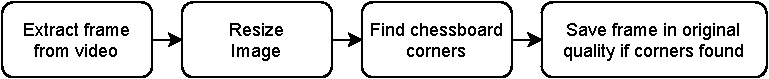
\includegraphics[width=\textwidth]{image/2/pipeline_2_1.pdf}
         \caption{Frame extractor algorithm}
         \label{fig:pipeline_vid}\par
         \vspace{6mm}
         
\includegraphics[width=\textwidth]{image/2/pipeline_2_2.pdf}
         \caption{Coefficient finder algorithm}
         \label{fig:pipeline_pic}
     \end{minipage}
\end{figure}

The two pipelines are kept separate, as this allows frames from the recording to be sorted and modified before they enter the next pipeline. This can be as simple as sorting out poor quality frames from a detection run up to optimising individual parameters in the pipeline itself without waiting too long to process all frames. In more advanced applications, however, these two pipelines can be combined.\\

\subsection{Frame extractor algorithm}\label{video_alg}

The algorithm starts to read in the recordings. Since the recordings are provided in the file format \textit{.h264} it needs to be taken care of to read them in correctly. For advanced applications can in this step further details be extracted from the recording like frames per seconds, total frame number, etc.\\

If the frames of the recording can be accessed, they are processed successively to find the interior corners of the checkerboard in the frames. So with a checkerboard of size 8x8 there are 7x7 interior corners present. \cite{cv} The result can be seen in figure \ref{fig:colour_corners}. The goal of this step is to find suitable images to calculate the intrinsic matrix in the next pipeline.\\

\begin{figure}[H]
    \centering
    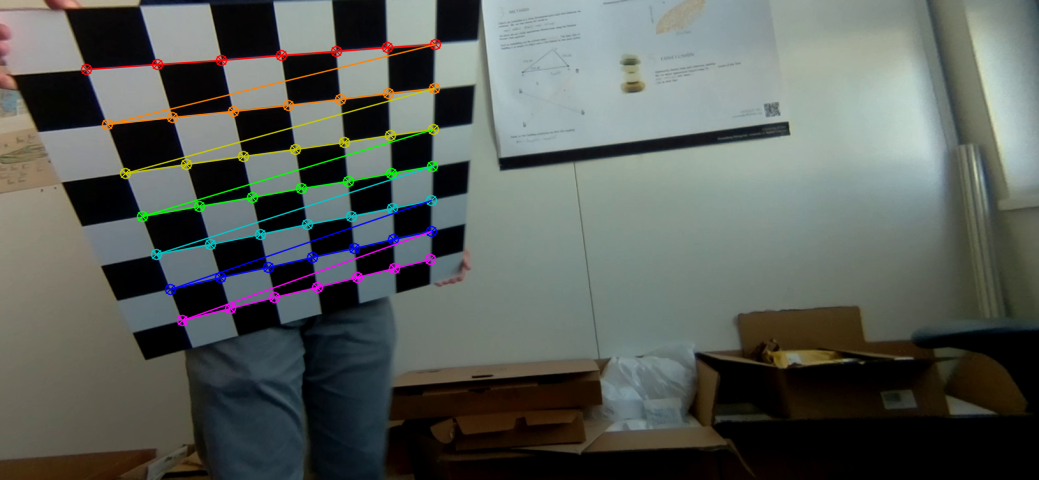
\includegraphics[width=.8\textwidth]{image/2/colour_corners.png}
    \caption{Found interior corners coloured in different colours}
    \label{fig:colour_corners}
\end{figure}

The functionality to extract the interior checkerboard corners has been developed by \textit{Vladimir Vezhnevets} \cite{vezhnevets}. One can find the implementation in \cite{vez_2}. A preprocessing step is taken beforehand which downscales the original 1920x1080 frame to a smaller resolution to cut off processing time. A deeper discussion about this topic can be seen in chapter \ref{experiment}.\\

One important feature is that the algorithm, which implements \textit{Vladimir Vezhnevets} algorithm, additionally accepts different flags that can be combined to add further filtration steps before the use of the algorithm of \textit{Vladimir Vezhnevets}. \cite{cv}\\

In this project the flag \textit{CALIB\_CV\_FAST\_CHECK} is used. "When this option is present, a fast scan will be done on the image to make sure that there actually are any corners in the image. If there are not, then the image is skipped entirely." \cite{cv} There are more flags available but because they all implemented or build up on top of an adaptive thresholding technique they are not considered here. Adaptive thresholding holds the risk to falsely cut off necessary information because of a set threshold value which is too high or too low for the image. This threshold value can not be changed in this flags. \\

Furthermore it is recommended to search for an asymmetric arrangement of interior corners of even and odd dimensions, here eg. 7x6. \cite{cv} "Using such even-odd asymmetry yields a checkerboard that has only one symmetry axis, so the board orientation can always be defined uniquely." \cite{cv}\\

\newpage

This recommendation is not used in this set of recordings because it had no effect on the rate of success of finding the checkerboard with interior corners of size 7x7 with searched for corner sizes of 7x7, 7x6 or 6x7. From a total amount of 2699 frames from all videos only 10 frames could be successfully detected with the these corner sizes, which correspond to 0.37\% of total found checkerboards. Even with a more robust method of finding the interior corners described in \cite{Geiger2012ICRA}, more checkerboards could not be found.\\

One possibility why with this corner sizes only a low amount of checkerboards were successfully found could be that the recordings of the checkerboard do not have a clear enough image of the checkerboard to be successfully detected with a corner size of 7x7. This means that the specifications for the detection of the corners in the algorithm itself are too strict to find all corners on the too noisy or blurred image.\\

Because of this consideration, an attempt was made to detect the checkerboard in the recordings with a corner size of 6x6. This resulted in 653 successfully found checkerboard frames, which correspond to 24.19\% of total found checkerboards. It can thus be concluded that the smaller the specified corner size, the more successfully found checkerboard frames there are. For a deeper discussion about this conclusion see chapter \ref{experiment}.\\

The last step of the algorithm is to save the frames with successfully found checkerboards into a separate folder. The images can be looked at, modified or sorted further for the next pipeline.\\
\vspace{-3mm}
\subsection{Corner size vs. image resolution}\label{experiment}

To even further determine how the checkerboard size effects the amount of successfully found images a series of tests were conducted. For this purpose, all 2699 frames were analysed with different corner sizes (7x7, 6x7, 7x6, 6x6) and the amount of successfully found images has been noted. Additionally, it was looked at how to make the process as a whole faster.\\

Since the checkerboard has clearly defined interior corners, these should also be easily recognisable in a resolution images. The advantage is that finding corner points takes much less processing time in a low resolution image in comparison to a high resolution image because fewer pixels need to be analyzed and looked through.\\

As a result of the recordings been recorded in a resolution of 1920x1080 the related aspect ratio of 16:9 was taken as a base to downscale the images to the same aspect ratio. This allows the content of the image to be retained in the downscaled version at the same length ratio as in the source image which can be an advantage in the next pipeline. Thus the following broad range of resolutions of nearly equal steps were chosen: 1280x720, 854x480, 640x360, 426x240 and 256x144.\\

The tests proceed accordingly to the algorithm that has been already mentioned in chapter \ref{video_alg}. All the frames of the videos are read in and an attempt is made to find the interior corners of the checkerboard. However, each frame is additionally reduced to all of the the different resolutions and with every resolutions to all of the different corner sizes.\\

Figure \ref{fig:exp_data} shows the result of the test runs. Three values were noted for each pair: total amount of elapsed processing time over all frames \textbf{(time)}, amount of successfully found checkerboards \textbf{(found)}, and the value \textit{successfully (found) frames per second} \textbf{(sfps)}.

\begin{figure}[H]
    \centering
    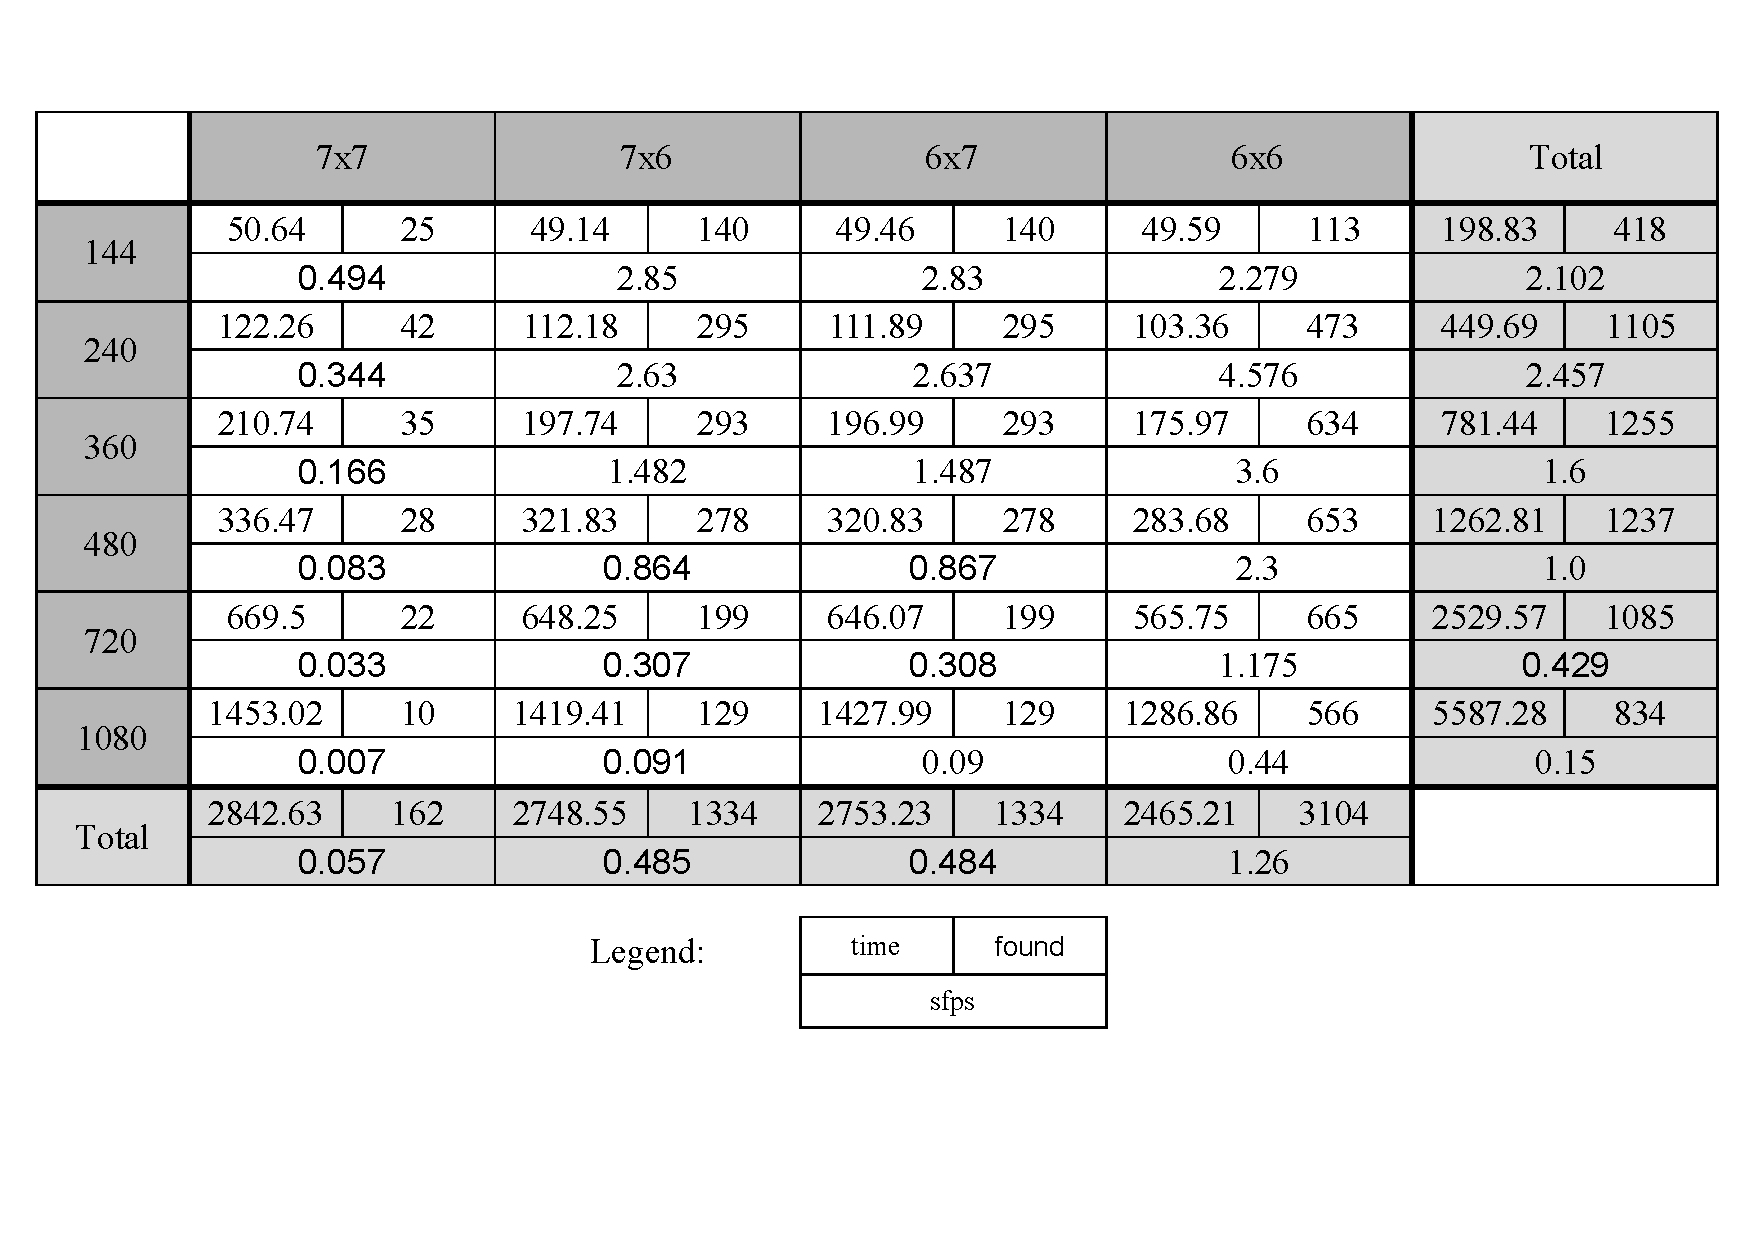
\includegraphics[width=.9\textwidth]{image/2/experiment_data.pdf}
    \caption{Collected Data from test runs}
    \label{fig:exp_data}
\end{figure}

A visualization of the raw collected data in figure \ref{fig:exp_data} can be seen in figure \ref{fig:exp}.

\begin{figure}[H]
    \centering
    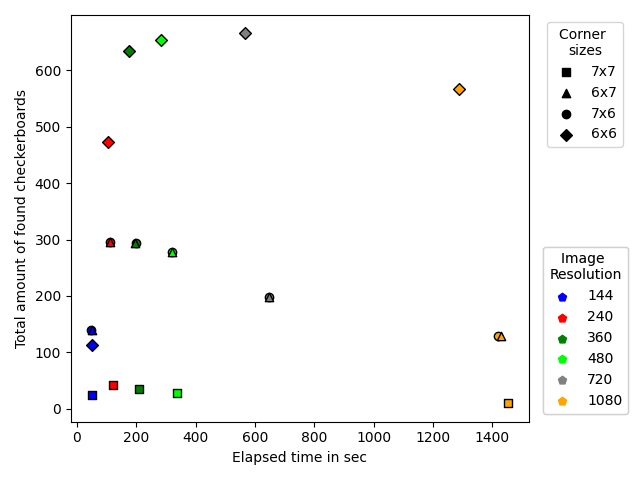
\includegraphics[width=.8\textwidth]{image/2/experiment.png}
    \caption{Visualisation of the collected data}
    \label{fig:exp}
\end{figure}

In figure \ref{fig:exp} one can see the following relations:
\begin{itemize}
    \item With a corner size of 7x7 the lowest total amount of successfully found checkerboards with all resolutions have been found. In figure \ref{fig:exp_data} this corner size has a total sfps of 0.057.
    \item The corner sizes of 6x7 and 7x6 are nearly identical in every resolution for the elapsed time and the total amount of successfully found checkerboards. In figure \ref{fig:exp_data} this corner sizes have a nearly identical sfps of 0.485 and 0.484 and the same total amount of successfully found checkerboards of 1334.
    \item For every corner size there is an image resolution range which includes the biggest total amount of successfully found checkerboards. This doesn't include both extreme points of 256x144 and 1920x1080. In figure \ref{fig:exp_data} the resolution 426x240 has the highest sfps of 2.457 and the resolutions 256x144 and 1920x1080 have the lowest total amount of successfully found checkerboards of 418 and 834.
    \item The image resolution of 256x144 has for all corner sizes the lowest total amount of successfully found checkerboards. In figure \ref{fig:exp_data} this resolution has the lowest total amount of successfully found checkerboards of 418.
\end{itemize}

One can argue that the resolution 256x144 has not the highest sfps overall like one can see in figure \ref{fig:exp_data}, but looking at individual corner sizes it has the highest sfps overall, except in the corner size of 6x6. However, this resolution is not recommended because in comparison to the resolution of 426x240. It has nearly for every corner size 50\% less successfully found checkerboards and in total 37\% less successfully found checkerboards. It can compensate for this circumstance by its overall lower processing time, in total 198.83 seconds, nearly half of the resolution of 426x240 with a processing time of 449.69 seconds. If choosing this resolution one should keep this in mind.\\

Likewise it is important to note that it is not known whether a poorer intrinsic matrices is produced if low resolution images of the source frame is used. In this project the successfully found high resolution frames are used in the second pipeline for the most detailed coefficients.\\

Furthermore it is important to note that the results depend heavily on the used images. The overall numbers in figure \ref{fig:exp_data} should be taken with a grain of salt. The trend of taken low resolution images to speed up the detection process and using a lower corner size than what is used to produce more successfully found checkerboards can be noted though.\\

From this follows that for this project a specified corner size of 6x6 will be used if no checkerboard frames with a specified corner size of 7x7, 7x6 or 6x7 could be found. Further as preprocessing step the source frame will be downscaled to the matching highest sfps of the used corner size, except with a resolution of 256x144. If a higher amount of successfully found checkerboards is needed then the next higher resolution shall be used. In the case of a corner size of 6x6 the frame will be downscaled to a resolution of 426x240 or 640x360.\\

\subsection{Coefficient finder algorithm}

The algorithm reads in the images, which there selected in the previous pipeline. With this images the checkerboard corners are to be detected and the found interior corner locations are saved in a separate list to use for the calculation of the intrinsic matrix. For that step the algorithm of chapter \ref{video_alg} is used.\\

\newpage

It is recommended to use at least "10 images of a 7 × 8 or larger chessboard" \cite{cv} to obtain high-quality results. \cite{cv} This is necessary because "consideration for noise and numerical stability is typically what requires the collection of more images of a larger chessboard." \cite{cv}\\ 

With these corner locations the intrinsic matrix can be calculated. For this purpose, the methodology in \cite{zhang2000} will be used. Additionally the distortion matrix needs to be calculated too. The methodology for this is described in \cite{brown} and \cite{brown_2}. \cite{cv}\\

To describe distortion effects radial distortion and tangential distortions are mainly used. "Radial distortions arise as a result of the shape of lens, whereas tangential distortions arise from the assembly process of the camera as a whole." \cite{cv} There are lot of different kinds of distortions, but they have a lesser effect on the overall distortion of an image than radial and tangential distortions. \cite{cv}\\

Radial distortion occurs near the edges of an image because "rays farther from the center of the lens are bent more than those closer in." \cite{cv} A typical lens is the so called \textit{fisheye} lens. This nonlinear behaviour from the optical center to the edge of the image sensor can be calculated with a Taylor series. "For cheap web cameras, we generally use the first two [...] terms; [...] For highly distorted cameras such as fisheye lenses, we can use a third radial distortion term." \cite{cv} This terms are labelled as $k_1,...,k_n$. \cite{cv}\\

Tangential distortions is "due to manufacturing defects resulting from the lens not being exactly parallel to the [image sensor] plane". \cite{cv} This distortion terms are labelled as $p_1$ and $p_2$. \cite{cv}\\

The question could arise why two separate models and therefore two sets of coefficients are needed. The intrinsic matrix describes the relation between the camera coordinate system and the pixel position on the image sensor plane. If a pinhole model is assumed, only the intrinsic matrix is needed to map the pixel positions to a 3D-line, which goes through the pinhole. \cite{cv} \cite{mat_calib}\\

However, modern cameras use a lens or a set of lenses in front of the image sensor. Through the use of these lenses additional offsets of the pixel to the 3D-line, depending on the pixel position on the image sensor plane, occur. \\

Depending on the type of camera, this can lead to the real world appearing skewed or twisted where eg. no easy distance calculations can be made about the real world without prior preparation of the image. \cite{cv} \cite{mat_calib}\\

For an example see figure \ref{fig:omni_cam}. To undo this distortion, so to know which pixel has to be moved where to straighten the edges, both matrices have to be used.

\begin{figure}[H]
    \centering
    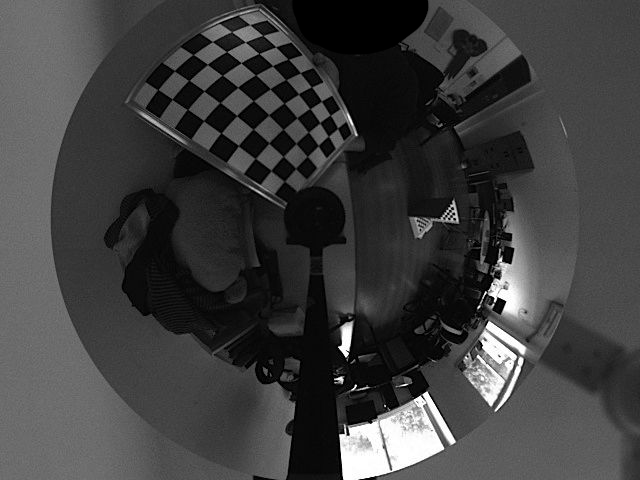
\includegraphics[width=.6\textwidth]{image/2/omnidirectional.png}
    \caption{The raw image of an omnidirectional camera\\Source: \cite{cv}}
    \label{fig:omni_cam}
\end{figure}

When both sets of coefficients are acquired the distorted image can be undistorted. For this purpose, the methodology described in \cite{distort_cv} is used. Through this process a new set of instructions is obtained which describes how every pixel has to be moved and scaled, a so called \textit{map}. \cite{distort_cv} \cite{remap} This remapping of the pixel can be seen in figure \ref{fig:map_remap}. \\

\newpage
\begin{figure}[H]
     \centering
     \captionsetup{justification=centering}
     \begin{minipage}[c]{0.5\textwidth}
        \centering
        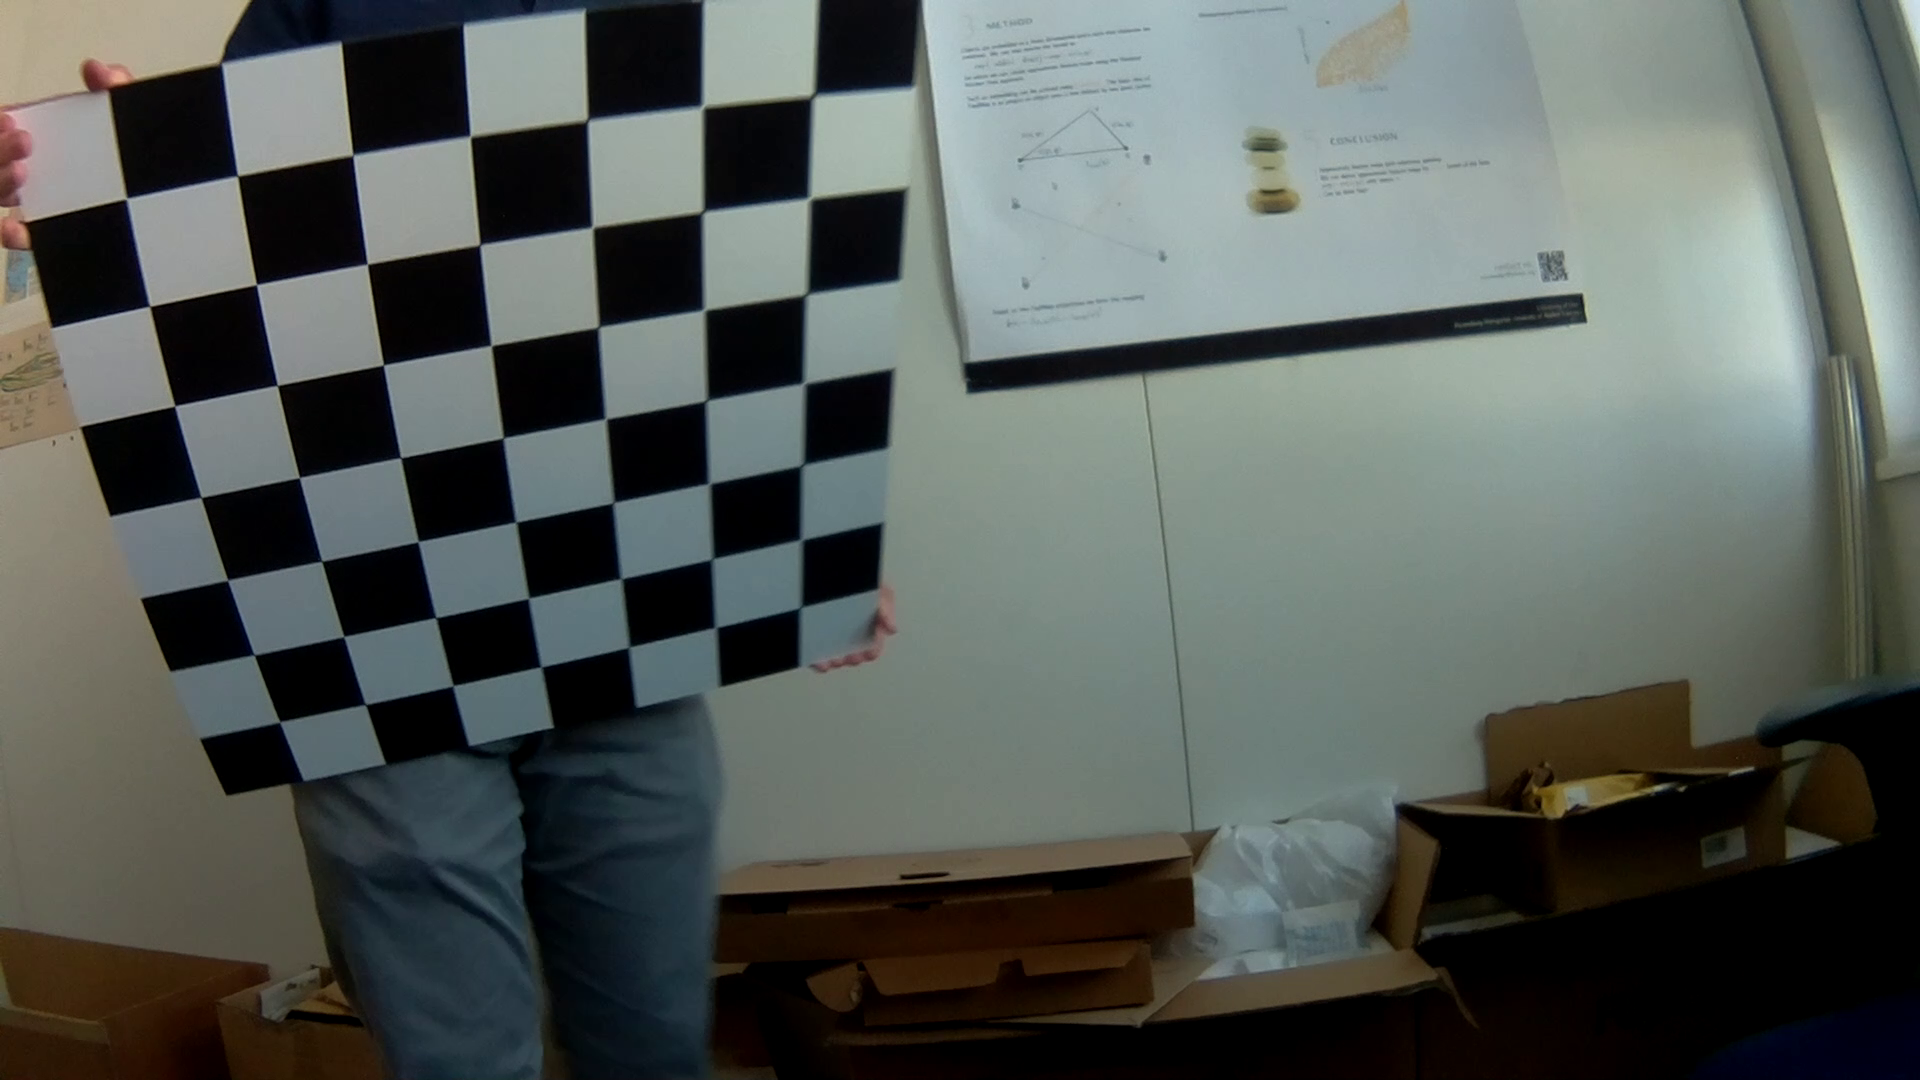
\includegraphics[width=.95\textwidth]{image/2/undist_og.png}
        \caption{Source frame}
        \label{fig:map_og}
     \end{minipage}%
     \begin{minipage}[c]{0.5\textwidth}
        \centering
        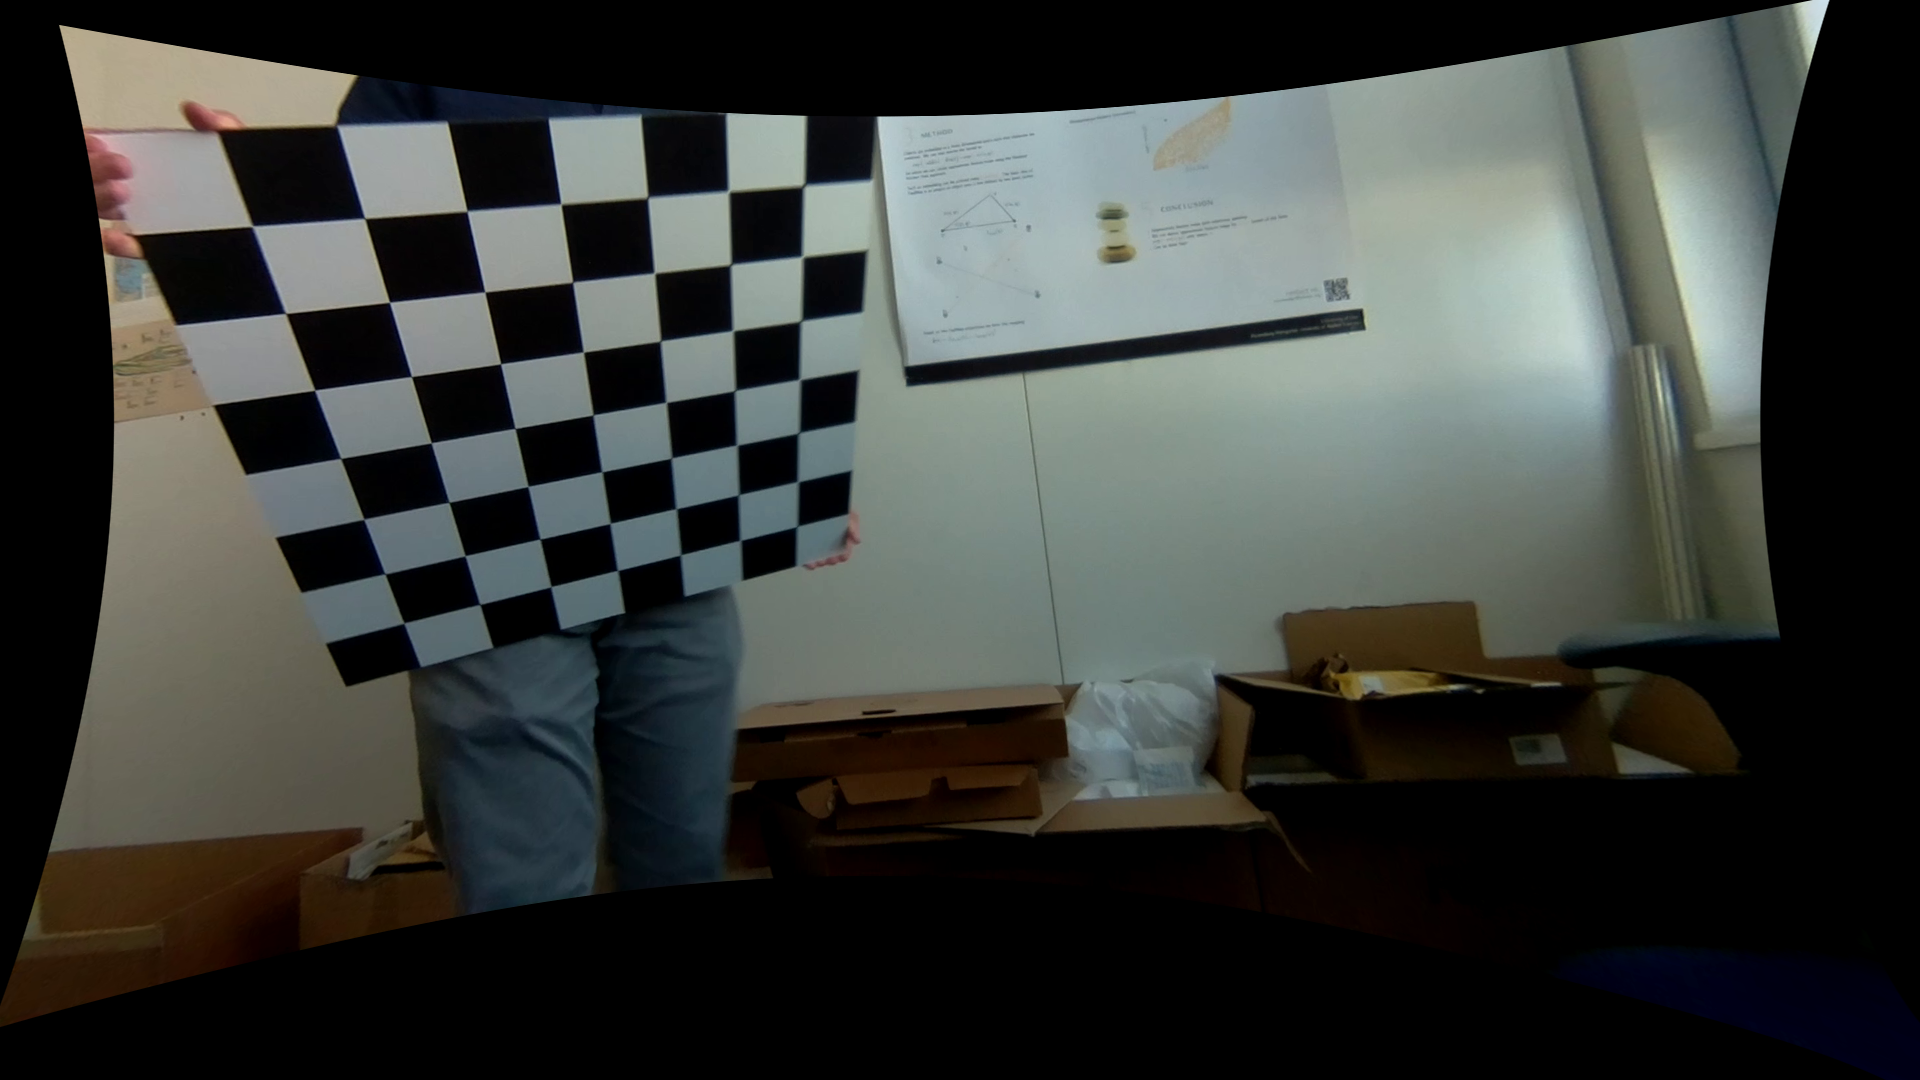
\includegraphics[width=.95\textwidth]{image/2/undist_without_roi.png}
        \caption{Remapped frame}
        \label{fig:map_remap}
     \end{minipage}
\end{figure}


It can be noted that this remapping creates black voids around the edges which is left to the user to decide how to crop the image accordingly to his desired output.
The easiest solution for this problem is to search for the nearest point of the one void to the center and cut the image parallel to the image edge of this void. The result can be seen in figure \ref{fig:dst_frame}. The disadvantage is that a lot of the non-black pixels in the corners are lost too. \\



